% latex packages to load.
\documentclass[12pt]{article}
\usepackage{geometry}
\geometry{a4paper}
%\geometry{landscape}
\usepackage[parfill]{parskip}    % Activate to begin paragraphs with an empty line rather than an indent
\usepackage{graphicx}
\usepackage{amssymb}
\usepackage{epstopdf}
\usepackage{fancyhdr}
\usepackage{fullpage}
\usepackage{appendix}
\usepackage{newclude}
\usepackage{datetime}
\usepackage{hyperref}
\usepackage{color}
\usepackage{multicol}
\usepackage{tabularx}
\usepackage{enumerate}
\usepackage{enumitem}
\usepackage{listings}
\usepackage{varwidth}
\usepackage{wallpaper}
\usepackage{lastpage}
\usepackage{titling}
%\usepackage{multind}
\usepackage[dutch]{babel}
\usepackage[table]{xcolor}
\usepackage{mathtools}
\usepackage{amsmath}
\usepackage{MnSymbol}
\usepackage{wasysym}

\usepackage[default,osfigures,scale=0.90]{opensans} %% Alternatively
%% use the option 'defaultsans' instead of 'default' to replace the
%% sans serif font only.
\usepackage[T1]{fontenc}

%tikz images, unquote to use block, color block, autograph block, cloud, line and line node
\usepackage[framemethod=tikz]{mdframed}
\usepackage{tikz}
\usetikzlibrary{shapes, arrows}

\tikzstyle{block} = [rectangle, draw, text width = 6em, text centered, rounded corners, minimum height = 4em]
\tikzstyle{colorblock} = [rectangle, draw, fill = blue!20, text width = 6em, text centered, rounded corners, minimum height = 4em]
%\tikzstyle{inputblock} = [rectangle, draw, text width = 24em, minimum height = 2.5em]
%\tikzstyle{autographblock} = [rectangle, draw, fill = black!1, text height = 0, text depth = 2cm, text width = 24em, minimum height = 8em]
\tikzstyle{cloud} = [ellipse, draw, minimum height = 4em]
\tikzstyle{line} = [draw, -latex']
\tikzstyle{line node} = [draw, fill = white]
\tikzstyle{decision} = [diamond, aspect=2, draw, text badly centered]

\usepackage[official]{eurosym}

\newcommand{\usemodule}[1]{\index{modules}{#1}\texttt{#1}}

\definecolor{gray}{rgb}{0.5,0.5,0.5}
\definecolor{tableheader}{rgb}{0.7,0.7,0.7}

\setlist[description]{style=nextline}
\renewcommand{\familydefault}{\sfdefault}

% link setup
\hypersetup{
    colorlinks,
    citecolor=black,
    filecolor=black,
    linkcolor=black,
    urlcolor=black,
}

\DeclareGraphicsRule{.tif}{png}{.png}{`convert #1 `dirname #1`/`basename #1 .tif`.png}

% usefull commands:
\newcommand{\seeref}[1]{\ref{#1} p.\pageref{#1}}
%\newcommand{\see}[1]{ (zie \ref{#1} p.\pageref{#1})}
\newcommand{\seesee}[2]{ (zie \ref{#1} p.\pageref{#1},  \ref{#2} p.\pageref{#2})}

% style for code blocks
\lstset{
    linewidth=1\textwidth,
    breaklines=true,
    numbers=left,                   % where to put the line-numbers
    numberstyle=\tiny\color{gray},  % the style that is used for the line-numbers
    stepnumber=1,                   % the step between two line-numbers. If it's 1, each line 
    numbersep=5pt, 
    basicstyle=\footnotesize,
}

% Header and Footer settings
\URCornerWallPaper{0.13}{img/dop/koptekstlogo.png}
\pagestyle{fancy}
\fancyhead{}
\renewcommand{\headrulewidth}{0pt}


\fancyfoot[L]{Drupal training}
\fancyfoot[C]{  }
\fancyfoot[R]{\textbf{\thepage}\ / \pageref{LastPage} \linebreak \linebreak \_\_\_\_\_\_\_ }

% Settings for table of contents.	
\setcounter{secnumdepth}{4}
\setcounter{tocdepth}{3}


\makeatletter
% some extra spacing for the table of contents
\renewcommand{\l@subsection}{\@dottedtocline{2}{1.5em}{3em}}
\renewcommand{\l@subsubsection}{\@dottedtocline{2}{2.7em}{4em}}

\renewcommand\paragraph{%
   \@startsection{paragraph}{4}{0mm}%
      {-\baselineskip}%
      {.5\baselineskip}%
      {\normalfont\normalsize\bfseries}}
\makeatother

% Define variables
\newcommand{\customer}{Dimpact}
\newcommand{\projectname}{Training}
\newcommand{\customerdomain}{Het klantdomein}
\newcommand{\authors}{E Lawende}


% Voorblad of the document
\ThisLRCornerWallPaper{0.8}{img/dop/voorbladlogo.png}

\title{\textbf{\customer} \\ \projectname}
\pretitle{\begin{flushleft}\LARGE}
\posttitle{\par\end{flushleft}}


\author{}  % skippen we voor maketitle
\date{}

% The actual Document:
\begin{document}
\maketitle
\vspace{-2.6cm}
\begin{flushright}
\begin{tabularx}{4.8cm}{ X }
Dutch Open Projects			\\
Doornseweg 12					\\	
3832 RL Leusden					\\
T: +31[0]33 - 4 50 50 50		\\
F: +31[0]33 - 4 50 50 57		
\\*
\\*
\\*
\\*
\\*
\\*
\\*
\\*
\\*
\\*
\\*
\\*
\\*
\\*
\\*
\\*
\\*
\\*
\footnotesize
\copyright All rights reserved.\\*
\footnotesize
No part of the contents of this publication may be reproduced, stored in a data processing system or transmitted in any form or by any means without the written permission of Dutch Open Projects B.V.
\end{tabularx}
\end{flushright}
  
 \null
 \vfill    
  \begin{tabularx}{\linewidth}{ p{4cm} X }
    Plaats & Leusden								\\
    Laatst bijgewerkt & \ddmmyyyydate \today		\\
    Auteurs & \authors							\\
    Versie & 1.1							\\
  \end{tabularx}
\pagebreak


% table of contents

\clearpage

\renewcommand*\contentsname{Inhoudsopgave}
\tableofcontents
\pagebreak

\section{Inhoud toevoegen}
\subsection{Typen inhoud}
Een website is in essentie opgebouwd uit inhoud, zoals een stuk tekst of een afbeelding, en verwijzingen naar deze inhoud, zoals in het hoofdmenu of een link in de tekst. Onderstaand screenshot geeft een willekeurige pagina waarin men dit terug kan zien:
\begin{center}
	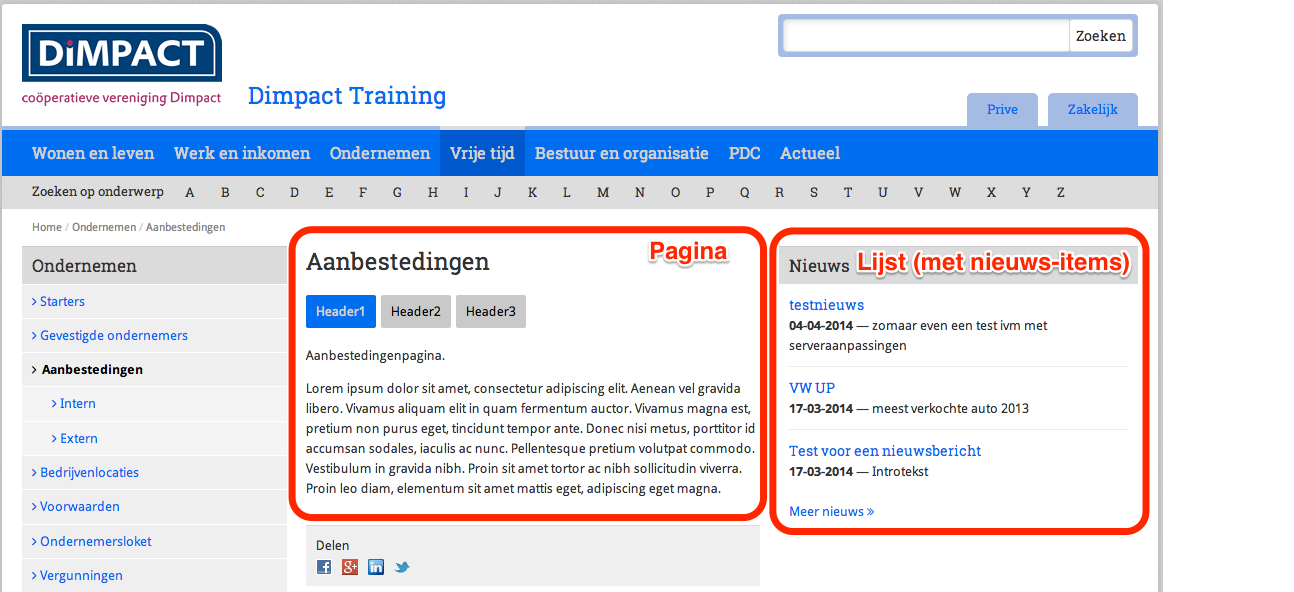
\includegraphics[scale=0.3]{img/inhoudstypen.png}
\end{center}
In het screenshot zien we --- naast het logo, diverse menu's en een zoekveld --- twee typen inhoud. Een pagina is misschien wel het meest elementaire type inhoud; het bestaat uit een stuk tekst, eventueel aangevuld met subkopjes, opmaak en afbeeldingen. Het screenshot geeft ook een lijst (of lijstblok) weer, met verwijzingen naar nieuws. Zowel een lijst als nieuws is een bepaald type inhoud.

Een aantal belangrijke inhoudstypen zijn:

\begin{tabular}{| l | p{12.6cm} |}
	\hline
	pagina & Een stuk tekst, eventueel aangevuld met subkopjes, opmaak en afbeeldingen. \\ \hline
	nieuws & Een nieuwsbericht. \\ \hline
	bestand & Een los bestand, zoals een afbeelding, dat via de website kan worden
		aangeboden c.q. weergegeven. \\ \hline
	agenda & Een agenda-item, bijvoorbeeld voor een bepaald evenement binnen de
		gemeente. \\ \hline
	peiling & Een vraag die aan bezoekers van de website wordt gesteld (ook wel poll
		genoemd). \\ \hline
	webformulier & Een formulier dat bezoekers van de website kunnen invullen (formulieren in Atos eSuite worden niet in Drupal geconfigureerd). \\ \hline
\end{tabular}

Er zijn nog diverse andere inhoudstypen. Een deel van de inhoud wordt ge�mporteerd. Producten, bekendmakingen en regelingen zijn hier een voorbeeld van. De volledige lijst met inhoudstypen is te vinden in de Dimpact-handleiding (\S2.8 'inhoudstypen').

\subsection{Workflow}
Bij het toevoegen van inhoud wordt een bepaalde workflow doorlopen, waarbij de status van de inhoud veranderd van 'concept' naar 'te beoordelen' naar 'gepubliceerd'. Dit is gekoppeld aan verschillende gebruikersrollen. Een redacteur kan een conceptversie aanmaken en deze ter beoordeling aanbieden aan de eindredacteur als de inhoud wat hem of haar betreft mag worden gepubliceerd. De eindredacteur kan deze inhoud vervolgens beoordelen en publiceren.

Later in de training volgt meer informatie over gebruikersrollen. De verschillende statussen van inhoud, en de workflow die deze doorloopt, is beschreven in de Dimpact-handleiding in \S2.2 ('workflow').

Om de status van inhoud te wijzigen klikt men in de adminbalk (de zwarte balk rechtsboven) op 'Mijn Workbench'. De pagina die nu verschijnt kent een aantal tabbladen, waaronder 'Mijn concepten' en 'Te beoordelen'.
\subsection{Scenario: nieuws-item toevoegen}
Deze paragraaf beschrijft een hands-on oefening waarbij een nieuws-item aan de website wordt toegevoegd. Het scenario wordt uitgevoerd door een redacteur en een eindredacteur.

\begin{enumerate}
\item Ga naar http://training.dimpact.dop.nu/user en log in als redacteur.
\item Ga met je muis in de adminbalk op \emph{Inhoud toevoegen} staan en kies \emph{Nieuws} uit de lijst met inhoudstypen die dan verschijnt.

\begin{center}
	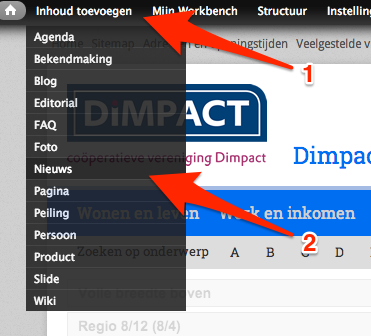
\includegraphics[scale=0.5]{img/new_content_news.png}
\end{center}

\item U komt nu in het venster \emph{Nieuws aanmaken}. Geef hier een titel op van het nieuwsitem.
\item Geef een intro op van het nieuws-item. Dit zijn de eerste paar regels van het nieuws-item, die vetgedrukt zullen worden weergegeven.
\item Geef de \emph{body} op. Dit is de volledige tekst van het nieuws-item. Merk op dat er mogelijkheden zijn om opmaak aan de tekst toe te voegen. Probeer bijvoorbeeld een woord te benadrukken door deze cursief weer te geven, maak een aantal \emph{bullet points} aan of voeg een link toe naar http://www.dop.nu/
\item Klik onder \emph{image} op de knop \emph{Selecteren}. Hiermee verschijnt het venster om een afbeelding toe te voegen (zie onder). Klik op \emph{Choose File} en kies een afbeelding om aan het nieuws-item toe te voegen.

\begin{center}
	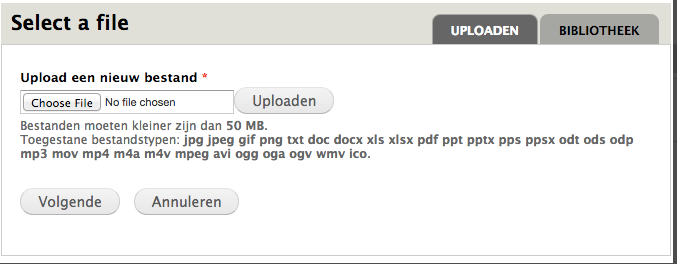
\includegraphics[scale=0.4]{img/file_chooser.png}
\end{center}

\item Klik op \emph{Uploaden} om het bestand op de server te plaatsen.
\item Klik op volgende.
\item U wordt gevraagd aan te geven of het gaat om een "publiek lokaal bestand aangeboden door de webserver"\ of een "\,afgeschermd lokaal bestand aangeboden via Drupal". In het eerste geval (publiek bestand) wordt het bestand benaderbaar via een herkenbaar adres (url), wat handig kan zijn als u hier van buitenaf naar wilt verwijzen. In dit geval gaat het om een afbeelding die bedoeld is om ergens op de website zelf te plaatsen (in dit geval bij een nieuws-item) en kiest u best voor de laatste optie ("\,afgeschermd lokaal bestand"). Klik op \emph{Volgende}.
\item Geef een \emph{Alt (alternative) Text} op voor de afbeelding. Deze tekst wordt weergegeven indien de afbeelding niet kan worden geladen, en wordt voorgelezen indien er gebruik wordt gemaakt van een \emph{screen reader} (voor blinden en slechtzienden).
\item Klik op \emph{Opslaan}.
\item Geef \emph{tags} (steekwoorden) op die betrekking hebben op het nieuws-item. U moet hier kiezen uit een bestaande lijst met mogelijkheden, en kunt hierbinnen zoeken door enkele letters in te typen. Onthoud welke \emph{tag} er is gebruikt; dit komt later in de training terug. U kunt meerdere \emph{tags} opgeven door deze te scheiden met een komma.
\item U kunt eventueel een locatie opgeven. In dit geval wordt er bij het nieuws-item een kaartje getoond.
\item Onderaan vindt u opties voor het publiceren van het nieuws-item. Ga naar \emph{Revisie-informatie} en pas de \emph{Moderatiestatus} aan naar \emph{Ter beoordeling}. Laat de overige opties op de standaardwaarden staan.

\begin{center}
	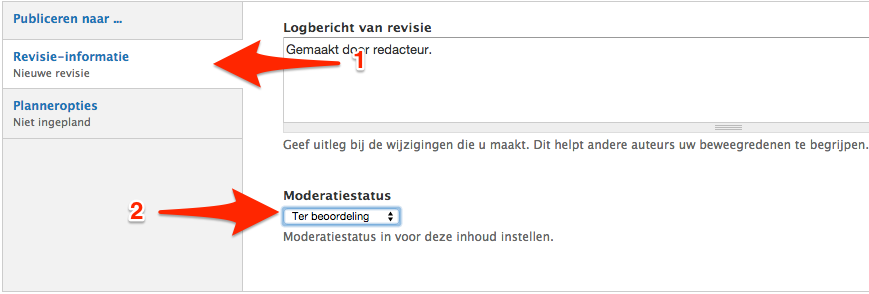
\includegraphics[scale=0.4]{img/publish.png}
\end{center}

\item Klik op \emph{Opslaan} om het nieuws-item te bewaren en, conform de zojuist opgegeven moderatiestatus, ter beoordeling aan te bieden aan de eindredacteur.

De redacteur is nu klaar met het toevoegen van een nieuws-item, maar deze staat nog niet op de website gepubliceerd. De rest van het scenario wordt uitgevoerd door de eindredacteur.

\item Log in als eindredacteur.
\item Klik in de adminbalk op \emph{Mijn Workbench} en ga vervolgens naar het tabblad \emph{te beoordelen}.
\item U ziet nu een lijst met het zojuist aangemaakte nieuws-item. Zie onderstaand screenshot voor een voorbeeld:

\begin{center}
	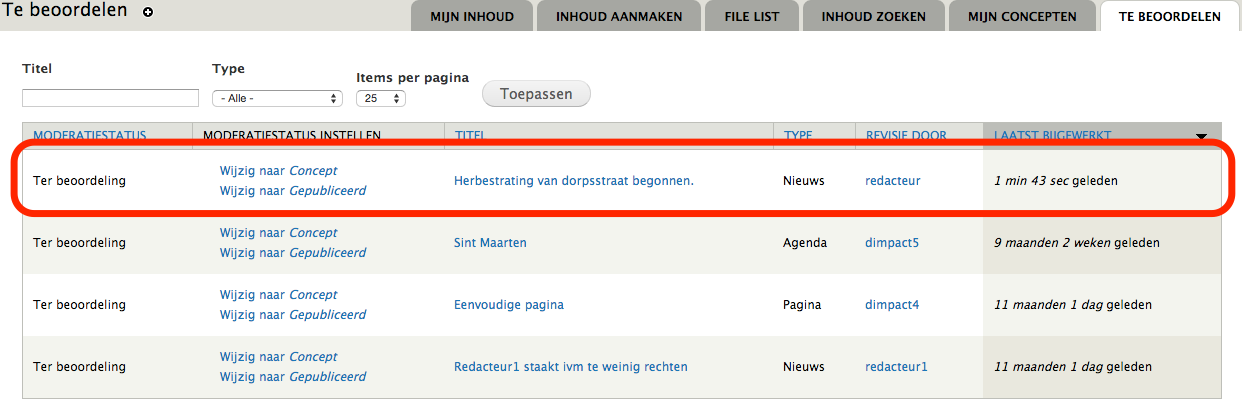
\includegraphics[scale=0.35]{img/te_beoordelen.png}
\end{center}

\item Klik op de titel van het nieuws-item om het te openen. Als eindredacteur kunt u nu beoordelen of de tekst geschikt is voor publicatie op de website.
\item Verander de moderatiestatus naar \emph{Gepubiceerd} en klik op \emph{Toepassen}.

\begin{center}
	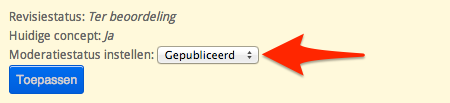
\includegraphics[scale=0.6]{img/publish2.png}
\end{center}

\item Het nieuws-item is nu gepubliceerd op de website. Aan de rechterkant staat een lijst met recent nieuws, waar het item ook is toegevoegd. Merk op dat hier, naast de titel, ook de introtekst wordt gebruikt.
\end{enumerate}

\subsection{Blokken}

Zoals eerder uitgelegd bestaat een webpagina uit verschillende stukken inhoud en navigatie. Als u een pagina bekijkt, zoals de thuispagina in onderstaand screenshot, dan kunt u hier diverse blokken onderscheiden. Tel bijvoorbeeld het aantal verschillende menu's dat u op deze pagina kunt vinden.

\begin{center}
	
\includegraphics[scale=0.5]{img/homepage.png}
\end{center}

Als u bent ingelogd ziet u ook lichtgrijze vlakken met daarin een tekst als "Volle breedte boven"\ of "Regio 8/12 (8/4)". Deze tekst verwijst naar een bepaalde regio en breedte. Wanneer u met de muisaanwijzer rechtsboven in een blok staat verschijnt een tandwieltje, zoals in onderstaand screenshot. Hier kunt u inhoud aan deze regio toevoegen.

\begin{center}
	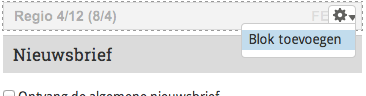
\includegraphics[scale=0.6]{img/felix.png}
\end{center}

In een blok kunnen diverse typen inhoud worden toegevoegd. De voornaamste typen zullen in deze training de revue passeren.

\subsection{Scenario: pagina en editorial toevoegen}

In dit scenario zal een pagina met een \emph{editorial} worden aangemaakt. Een editorial is een stukje content dat als blok aan een pagina kan worden toegevoegd.

\begin{enumerate}
\item Log in als eindredacteur of administrator.
\item Kies in de adminbalk voor \emph{Inhoud toevoegen} en vervolgens voor \emph{Editorial}. U krijgt nu een pagina die vergelijkbaar is met de pagina voor het toevoegen van een nieuws-item.
\item Geef een titel op, bijvoorbeeld "Meer informatie over x".
\item Geef tekst op in de body, bijvoorbeeld een externe link.
\item Zorg ervoor dat \emph{Gepubliceerd} is aangevinkt bij de publicatie-opties.
\item Klik op \emph{Opslaan}.
\item Kies in de adminbalk voor \emph{Inhoud toevoegen} en vervolgens voor \emph{Pagina}.
\item Maak een pagina aan en publiceer deze. Gebruik een titel die u kunt onthouden. Geef eventueel ook tags op, zoals de tags die u ook hebt gebruikt voor het nieuws-item.
\item U hebt nu een pagina aangemaakt waar de editorial kan worden toegevoegd. Open deze pagina en ga met de muisaanwijzer naar het tandwiel binnen het blok "Regio 4/12 (3/5/4) Node", rechts op de pagina. Klik op het tandwiel en kies \emph{Blok toevoegen}.

\begin{center}
	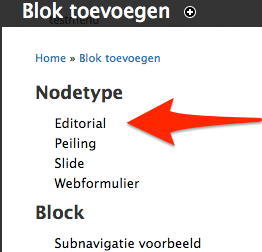
\includegraphics[scale=0.6]{img/add_block.png}
\end{center}

\item Kies voor \emph{Editorial} en vervolgens voor \emph{Volledige inhoud}.
\item Zoek en selecteer de eerder aangemaakte editorial. Deze staat waarschijnlijk boven in de lijst.
\item De editorial verschijnt rechts op de pagina, met de eerder opgegeven titel. U kunt deze aanpassen door de eigenschappen van dit blok aan te passen, zoals in onderstaand screenshot:

\begin{center}
	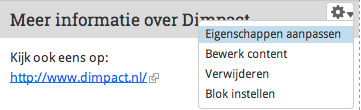
\includegraphics[scale=0.6]{img/felix_properties.png}
\end{center}

\item Vul "Meer info"\ in als onderwerp.
\item De editorial verschijnt rechts van de pagina.

\begin{center}
	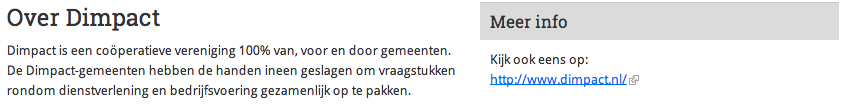
\includegraphics[scale=0.5]{img/editorial.png}
\end{center}

\end{enumerate}

\pagebreak

\section{Navigatie}
\subsection{Menu's}
De website bevat diverse menu's om snel naar de juiste informatie te kunnen navigeren. Onderstaand screenshot bevat een overzicht van de menu's op de trainingsomgeving:

\begin{center}
	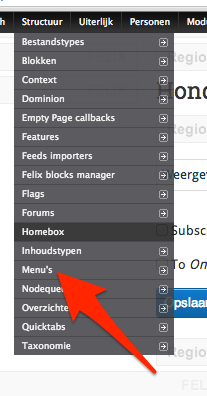
\includegraphics[scale=0.4]{img/menus.png}
\end{center}

Een volledige lijst van de menu's op de website kan worden opgevraagd door in de adminbalk naar \emph{Structuur} te gaan en vervolgens naar \emph{Menu's}. Wanneer achter een menu op \emph{links weergeven} wordt geklikt, wordt een lijst gegeven van alle items in het desbetreffende menu.

\begin{center}
	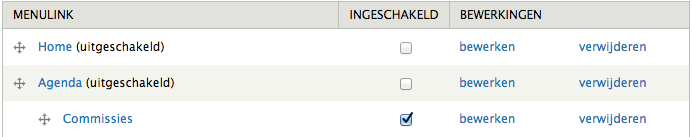
\includegraphics[scale=0.6]{img/menu_show_links.png}
\end{center}

In dit overzicht kan de volgorde binnen het menu worden aangepast (door te slepen) en kunnen menu-items tijdelijk worden uitgeschakeld. Uitgeschakelde menu-items zijn niet langer gepubliceerd, maar kunnen via dit overzicht eenvoudig worden teruggezet.

\subsection{Scenario: menu-item aanmaken}
Binnen dit scenario zal de eerder aangemaakte pagina aan het hoofdmenu worden toegevoegd.

\begin{enumerate}
\item Ga via de adminbalk naar \emph{Structuur} en vervolgens naar \emph{Menu's}.
\item Zoek binnen dit overzicht naar \emph{Main menu} en klik vervolgens op \emph{link toevoegen} in de laatste kolom.
\item Geef een titel op voor het menu-item.
\item Het pad geeft aan waar het menu-item naar verwijst. Klik op de knop \emph{Zoeken} achter dit veld.
\item Voer in het veld \emph{Search for content} (een deel van) de titel op van de pagina die in het vorige scenario is aangemaakt. Selecteer vervolgens deze pagina uit de lijst met zoekresultaten.
\item Klik op \emph{Link invoegen}.
\item Verder op de pagina staat een keuzeveld met de titel \emph{Bovenliggend onderdeel}. U kunt hier aangeven dat het toe te voegen menu-item een sub-item moet zijn van een ander item in het menu. Let op dat het keuzeveld alle items in alle menu's weergeeft. Laat het veld staan op "<Hoofdmenu>".
\item Laat de overige instellingen op hun standaardwaarden staan. Klik op \emph{Opslaan}.
\item Klik op het thuispagina-icoon helemaal linksboven. U ziet nu het zojuist toegevoegde menu-item.

\begin{center}
	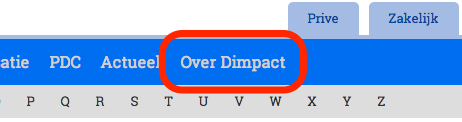
\includegraphics[scale=0.6]{img/added_menu_item.png}
\end{center}

\item Ga in de adminbalk terug naar \emph{Structuur}, \emph{Menu's}.
\item Klik op \emph{links weergeven} achter \emph{Main menu}.
\item Zoek het zojuist toegevoegde menu-item (deze staat waarschijnlijk helemaal onderaan) en klik op verwijderen.
\item Er wordt gecontroleerd of het menu-item ook in andere menu's voorkomt. Wanneer er wordt gevraagd om het item ook van andere menu's te verwijderen, selecteer dan alle opties en klik op \emph{Bevestigen}.
\end{enumerate}

\subsection{Lijsten en nodequeues}

Op de voorpagina zijn diverse afbeeldingen te vinden --- allen voorzien van een titel en achterliggende pagina. Deze afbeeldingen zijn als inhoud toegevoegd, met \emph{slide} als inhoudstype.

\begin{center}
	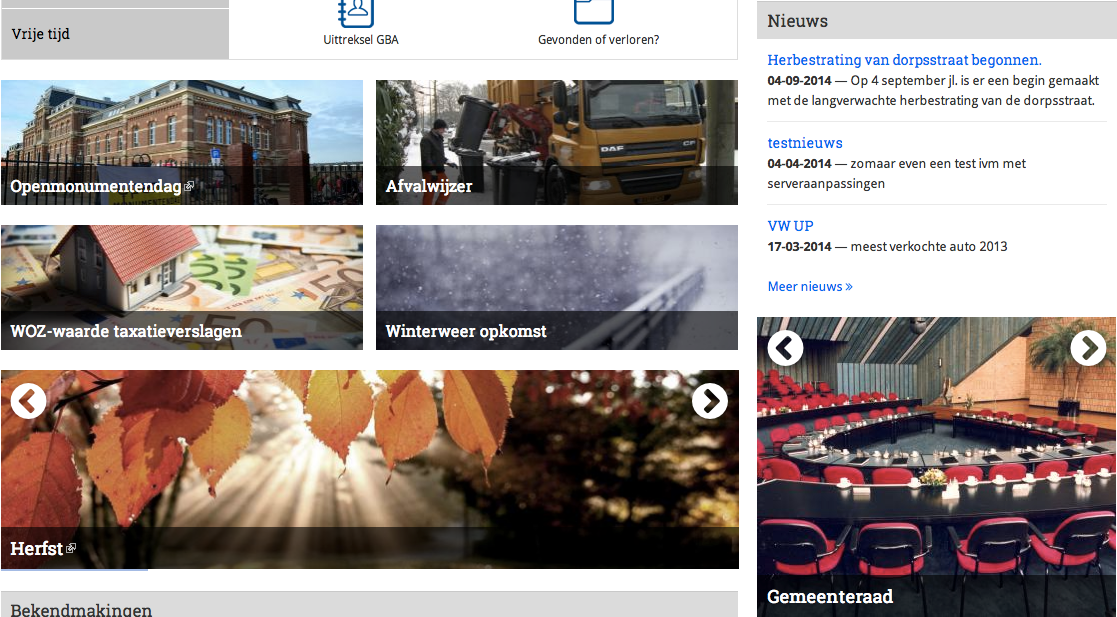
\includegraphics[scale=0.4]{img/frontpage_nodequeues.png}
\end{center}

Welke afbeeldingen er in een blok worden getoond is gedefinieerd in een \emph{nodequeue}. Een \emph{nodequeue} is een geordende lijst met inhoud. Deze inhoud hoeft niet het type \emph{slide} te hebben; het is bijvoorbeeld ook mogelijk een \emph{nodequeue} aan te maken die naar pagina's verwijst.

Het systeem kent ook een \emph{list}, wat een lijst is die dynamisch wordt opgesteld aan de hand van bepaalde criteria; het is bijvoorbeeld mogelijk een \emph{list} aan te maken van alle inhoud van het type \emph{slide}, waar een bepaalde tag aan is toegevoegd. Een lijst kan ook worden gekoppeld aan een \emph{nodequeue}, zodat een \emph{nodequeue} als pagina of als blok kan worden toegevoegd.

\subsection{Scenario: carrousel aanpassen}
Binnen dit scenario zult u \'{e}\'{e}n van de carrousels op de voorpagina aanpassen (dit zijn de afbeeldingen die om de paar seconden worden gewisseld). U zult hiervoor een \emph{slide} moeten aanmaken, en deze vervolgens toevoegen aan een \emph{nodequeue}.

\begin{enumerate}
\item Log in als beheer.
\item Ga naar de pagina waar de \emph{slide} naar moet verwijzen. Kopi\"{e}er of onthoud het laatste gedeelte van het webadres (url), bijvoorbeeld "\,/herbestrating-van-dorpsstraat-begonnen".
\item Kies in de adminbalk voor \emph{Inhoud toevoegen} en vervolgens voor \emph{Slide}.
\item Geef een titel op. Dit is de tekst die onder de foto zal verschijnen.
\item Geef het webadres uit stap 1 op bij \emph{Link}.
\item Selecteer een afbeelding. U kunt een eerder gebruikte afbeelding gebruiken door onder \emph{Image} op \emph{Selecteren} te klikken, en vervolgens naar het tabblad \emph{Bibliotheek} te gaan. Selecteer hier de gewenste afbeelding en klik onderaan op \emph{Indienen}.
\item Zet bij de publicatie-opties de moderatiestatus op \emph{gepubliceerd} en sla de slide op.
\item Ga nu in de adminbalk naar \emph{Structuur} en vervolgens naar \emph{Nodequeue's}. U krijgt nu een lijst met de nodequeues die in het systeem staan geconfigureerd. Wij zullen hier "Carrousel 4/12"\ gebruiken, die wordt gebruikt voor de carrousel rechtsonder op de thuispagina.
\item Klik achter "Carrousel 4/12"\ op \emph{Weergeven}. U ziet nu een lijst van de slides in de carrousel.
\item Gebruik het veld onder de tabel om de zojuist aangemaakt slide op te zoeken, en klik vervolgens op \emph{Inhoud toevoegen}.
\item Klik op \emph{Opslaan}.
\item Gebruik de knop helemaal linksboven om terug te keren naar de thuispagina.
\item Blader door de carrousel rechtsonder op de pagina. Staat de zojuist toegevoegde slide in de lijst?
\end{enumerate}

\begin{center}
	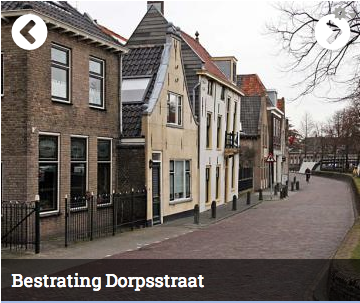
\includegraphics[scale=0.4]{img/carrousel.png}
\end{center}

\subsection{Tags}
Eerder in de training heeft u tags toegevoegd aan een nieuws-item en een pagina. Bij het toevoegen van deze tags heeft u moeten kiezen uit een lijst. Deze lijst staat opgeslagen als een \emph{taxonomie} (woordenlijst). U kunt woordenlijsten aanpassen door in de adminbalk te kiezen voor \emph{Structuur} en vervolgens voor \emph{Taxonomie}. Er verschijnt vervolgens een overzicht van de woordenlijsten in het systeem, waaronder de tags:

\begin{center}
	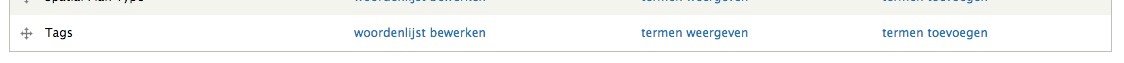
\includegraphics[scale=0.4]{img/taxonomy_tags.png}
\end{center}

\subsection{Scenario: inhoud met bepaalde tag}
In dit scenario zal bij een bepaalde pagina een lijst worden geplaatst, met inhoud waar een bepaalde tag aan is toegevoegd.

\begin{enumerate}
\item Ga in de adminbalk naar \emph{Structuur} en klik vervolgens op \emph{Lijsten}. U krijgt een overzicht van de lijsten in het systeem.
\item Klik op lijst toevoegen.
\item Geef een \emph{Administration title} en \emph{Titel} op voor de lijst.
\item Bij \emph{Instellingen} kunt u aangeven welke inhoud (\emph{nodes} in Drupal) in de lijst moet komen. U kunt hier bijvoorbeeld kiezen dat het moet gaan om een bepaald inhoudstype, zoals nieuws. Vul dit keer alleen een term in, en gebruik hiervoor de tag die eerder aan het nieuws-item is toegevoegd.

\begin{center}
	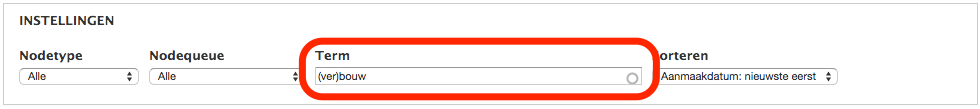
\includegraphics[scale=0.4]{img/list_term.png}
\end{center}

\item Vink \emph{Blok aanbieden} aan, binnen de sectie \emph{Blok}.
\item De weergavemodus geeft aan hoe de lijst wordt weergegeven. Het is bijvoorbeeld mogelijk om een deel van de inhoud in de lijst weer te geven, door te kiezen voor \emph{Teaser}. Laat in dit geval de waarde staan op \emph{Titles as link}.
\item Het aantal items geeft aan hoeveel links er maximaal in het blok worden weergegeven. Laat deze waarde staan op 5.
\item Vink \emph{Pagina aanbieden} uit; de lijst hoeft nu alleen als blok te worden toegevoegd.
\item Klik op \emph{Opslaan}.
\item Ga naar een pagina, zoals de pagina die u eerder in de training heeft aangemaakt, en kies \emph{Blok toevoegen} (u heeft dit eerder gedaan bij het toevoegen van een \emph{editorial}, in \S1.5).
\item Kies onder \emph{Custom Lists} voor de lijst die u zojuist heeft toegevoegd.

\begin{center}
	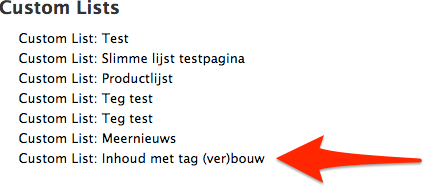
\includegraphics[scale=0.4]{img/custom_list.png}
\end{center}

\item Vul het onderwerp in. Dit is de titel die bovenin het blok wordt weergegeven.
\item Klik op \emph{Opslaan}.
\item De lijst is nu aan de pagina toegevoegd.
\end{enumerate}

\pagebreak

\section{Meer over Drupal en Dimpact}
Meer informatie over Drupal en Dimpact is te vinden in de handleidingen die in de training zijn aangereikt. Bekijkt u bijvoorbeeld het hoofdstuk over webformulieren in de Dimpact-handleiding. U vindt hier instructies over het aanmaken van formulieren op de website (die niet in Atos eSuite zitten). Let er op dat in deze formulieren niet naar persoonsgegevens wordt gevraagd.

Hoofdstuk 3 in de Dimpact-handleiding (\emph{User Management}) bevat informatie over gebruikers en gebruikersrechten, die voor beheerders relevant is.

De Drupal-handleiding bevat informatie over Drupal, die niet specifiek is voor Dimpact. Een nuttige functionaliteit die hier wordt beschreven is \emph{Masquerade}, in het hoofdstuk \emph{Personen}. Deze functionaliteit kan voor beheerders nuttig zijn en is op Dimpact-websites onderaan de pagina te vinden (mits u als beheerder bent ingelogd).

\end{document}
